\documentclass[14pt, fleqn, xcolor={dvipsnames, table}]{beamer}
\usepackage[T2A]{fontenc}
\usepackage[utf8]{inputenc}
\usepackage[english,russian]{babel}
\usepackage{amssymb,amsfonts,amsmath,mathtext}
\usepackage{cite,enumerate,float,indentfirst}
\usepackage{cancel}

\usepackage{tikz}                   
\usetikzlibrary{shadows}

% \usepackage{enumitem}
% \setitemize{label=\usebeamerfont*{itemize item}%
%   \usebeamercolor[fg]{itemize item}
%   \usebeamertemplate{itemize item}}

\graphicspath{{images/}}

\usetheme{Madrid}
\usecolortheme{seahorse}
\renewcommand{\CancelColor}{\color{red}}

\setbeamercolor{footline}{fg=Blue!50}
\setbeamertemplate{footline}{
  \leavevmode%
  \hbox{%
  \begin{beamercolorbox}[wd=.333333\paperwidth,ht=2.25ex,dp=1ex,center]{}%
    И. Кураленок, Н. Поваров, Яндекс
  \end{beamercolorbox}%
  \begin{beamercolorbox}[wd=.333333\paperwidth,ht=2.25ex,dp=1ex,center]{}%
    Санкт-Петербург, 2013
  \end{beamercolorbox}%
  \begin{beamercolorbox}[wd=.333333\paperwidth,ht=2.25ex,dp=1ex,right]{}%
  Стр. \insertframenumber{} из \inserttotalframenumber \hspace*{2ex}
  \end{beamercolorbox}}%
  \vskip0pt%
}
\newcommand\indentdisplays[1]{%
     \everydisplay{\addtolength\displayindent{#1}%
     \addtolength\displaywidth{-#1}}}
\newcommand{\itemi}{\item[\checkmark]}

\title{Машинное обучение: сэмплирование\\\small{}}
\author[]{\small{%
И.~Куралёнок,
Н.~Поваров}}
\date{}

\begin{document}

\begin{frame}
\maketitle
\small
\begin{center}
\vspace{-60pt}
\normalsize {\color{red}Я}ндекс \\
\vspace{80pt}
\footnotesize СПб, 2013
\end{center}
\end{frame}

\section{Содержание}
\begin{frame}{Содержание}
\begin{enumerate}
  \item Понятие сэмплирования
  \begin{itemize}
   \item Процесс сэмплирования;
   \item Основные методы сэмплирования.
  \end{itemize}
  \item Переборные методы в ML
  \begin{itemize}
   \item Полный перебор.
  \end{itemize}
  \item Hill climbing
  \item Сэмплирование марковскими цепями
  \begin{itemize}
   \item Metropolis-Hastings алгоритм;
   \item Алгоритм Гиббса.
  \end{itemize}
  \item Построение вероятностного пространства для максимизации
\end{enumerate}
\end{frame}

\begin{frame}{Понятие сэмплирования}
\textit{Сэмплирование} --- метод исследования множества путём анализа его подмножеств. \\
Применяется:
\begin{itemize}
   \item множество слишком велико для перебора;
   \item каждое дополнительное измерение дорого;
   \item предварительный анализ.
\end{itemize}
\end{frame}

\begin{frame}{Алгоритм сэмплирования}
\begin{enumerate}
   \item Понять какое множество мы изучаем;
   \item Осознать что из этого множества мы можем измерить;
   \item Определить количество измерений;
   \item Разработать план сэмплирования;
   \item Провести сэмплирование.
\end{enumerate}
\end{frame}

\begin{frame}{Типы сэмплирования}
\begin{itemize}
   \item Вероятностное сэмплирование: 
   $$
   p(x),\forall x:p(x) > 0
   $$
   \textit{Например: попробуем посчитать соотношение мужчин/женщин}
   \item Невероятностное сэмплирование:
   $$
   p(x), \exists x: p(x) = 0
   $$
   \textit{Например: попробуем посчитать безработных в рабочее время}
   \item Без возвращений;
   \item С возвращениями.
\end{itemize}
\end{frame}

\begin{frame}{Виды сэмплирования}
\begin{itemize}
   \item Вероятностное сэмплирование
   \begin{itemize}
    \item Простое вероятностное
    \item Систематическое
    \item Стратифицированное
    \item Пропорциональное
    \item Кластерное
   \end{itemize}
   \item Невероятностное сэмплирование
   \begin{itemize}
    \item Опрос ближайших
    \item Панельное сэмплирование
   \end{itemize}
\end{itemize}
\end{frame}


\begin{frame}{Как выбрать нужное?}
Надо учитывать:
\begin{itemize}
   \item природа и размер возможного сэмпла;
   \item наличие дополнительной информации об элементах;
   \item необходимя точность измерений;
   \item точность отдельных измерений в сэмплировании;
   \item стоимость измерений;
\end{itemize}
\end{frame}

\begin{frame}{Возвращаясь к ML}
$$
F_0 = \arg\max_F p(F|X)
$$
\begin{description}
  \item[\color{green}+] если известны вероятности можно попробовать посэмплировать решения;
  \item[\color{red}---] не определено пространство F;
  \item[\color{red}---] неясно как устроить обход.
\end{description}
\end{frame}

\begin{frame}{Иногда все просто}
$$
F_0 = \arg\max_{F \in \{f_i\}_{i=1}^n} p(F|X)
$$
\begin{enumerate}
  \item введём порядок обхода;
  \item переберём все возможные решение;
  \item составим взвешенное решение/выберем лучшее.
\end{enumerate}
\end{frame}

\begin{frame}{Но чаще всё непросто}
$$
F_0 = \arg\max_{F \in \{f_i\}_{i=1}^\infty} p(F|X)
$$
\begin{enumerate}
  \item введём порядок обхода;
  \item применим систематическое сэмплирование;
  \item составим взвешенное решение/выберем лучшее.
\end{enumerate}
\end{frame}

\begin{frame}{Случайное блуждание I}
Чтобы построить порядок обхода можно воспользоваться такой схемой:

$$\begin{array}{l}
F = F(x, \lambda), \lambda \in \mathcal(R)^n \\
F_t = F(x. \lambda_t) \\
\lambda_{t+1} = \lambda_t + \xi~~~~C(\lambda_{t+1} | \{\lambda_i\}_0^t) \\
\end{array}$$

\begin{itemize}
  \item будем блуждать по пространству параметров;
  \item необходимо определить:
  \begin{enumerate}
    \item способ сделать шаг;
    \item условие принятия этого шага.
  \end{enumerate}
\end{itemize}
\end{frame}

\begin{frame}{Случайное блуждание II}
На что стоит обратить внимание при построении блуждания:
\begin{itemize}
  \item размерность $\lambda$ может быть меньше чем кажется;
  \item ограничения на $\lambda$ существенно осложняют процедуру.
\end{itemize}
\end{frame}


\begin{frame}{Некоторые виды случайного блуждания}
\begin{itemize}
  \item множество фиксированных шагов $\xi \sim U(\{\xi_i\}_1^m)$;
  \item гауссовское $\xi_i \sim N(\mu, \sigma^2)$;
  \item самозависимое;
  \item etc.
\end{itemize}
\end{frame}

\begin{frame}{Simple hill climbing}
$$\begin{array}{l}
\xi \sim U(\{\xi_i\}), \xi_{ii} = \omega, \xi_{ij} = 0, j \neq i,\\
\\
C(\lambda_{t+1}|\lambda_t) = \frac{p(F(\lambda_{t+1})|X)}{p(F(\lambda_t)|X)} > 1 \\
\end{array}$$
Свойства:
\begin{itemize}
  \item простой;
  \item быстро сходится;
  \item зависим от выбора начальной точки.
  \item etc.
\end{itemize}
\end{frame}

\begin{frame}{Random-restart (shotgun) hill climbing}
\begin{center}
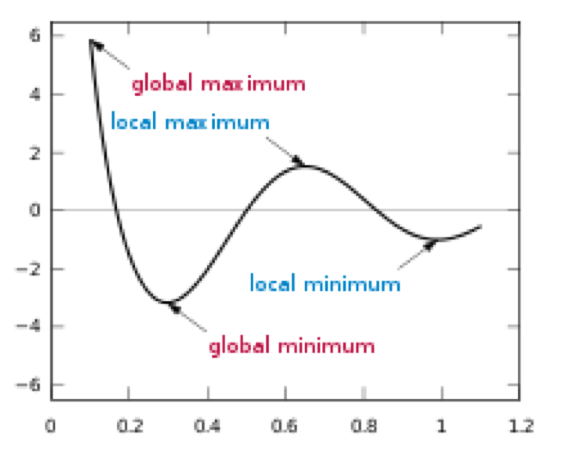
\includegraphics[width=0.4\textwidth]{hill_climb.png}
\end{center}
\footnotesize
Проблемы:
\begin{itemize}
  \item сходится в локальный максимум;
  \item может долго сходиться, если начало далеко от максимума;
  \item аллеи.
\end{itemize}
$\Rightarrow$ Можно рестартить hill climbing из разных начальных точек
\end{frame}

\begin{frame}{Интуиция}
\begin{itemize}
  \item наверное нельзя всегда ходить ''по шерсти'';
  \item хорошо бы обойти всё пространство;
  \item скорость движения должна меняться.
\end{itemize}
$\Rightarrow$ Markov Chain Monte-Carlo (MCMC)
\end{frame}

\begin{frame}{Metropolis-Hastings алгоритм}
$$\begin{array}{l}
p(\lambda|\lambda_t)\\
\\
\alpha = \frac{p(F(\lambda_t)|X)p(\lambda_t|\lambda)}{p(F(\lambda)|X)p(\lambda|\lambda_t)}\\
\\
\psi \sim U(0,1)\\
\\
C(\lambda_{t+1}|\lambda_t) = \left\{  
           \begin{array}{rcl}  
            1, \alpha \ge \psi \\  
            0 \\  
           \end{array}   
           \right.  
\end{array}$$
Например, $p(\lambda|\lambda_t) \sim N(\lambda_t|\sigma^2E)$
\end{frame}

\begin{frame}{Свойства}
\begin{center}
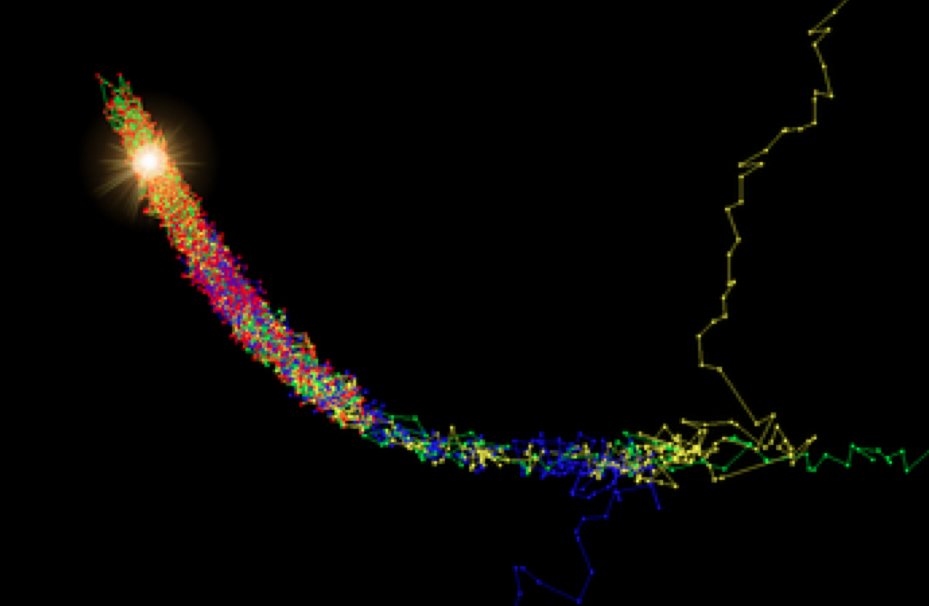
\includegraphics[width=0.5\textwidth]{mcmc.png}
\end{center}
\footnotesize
Доказано:
\begin{itemize}
  \item обходит всё пространство;
  \item это действительно взвешенное сэмплирование;
\end{itemize}
$\Rightarrow$ точно придём в максимум! \\
Проблема только с тем, что придём за бесконечное время
\end{frame}

\begin{frame}{Алгоритм Гиббса}
В Метрополисе есть проблема: всё зависит от $p(\lambda|\lambda_t)$.
$$\begin{array}{l}
i \sim U(1, ..., n) \\
\\
p(\xi|\lambda_t) \\
\\
\lambda_i = \lambda_{t_i} + \xi, \\
\\
\lambda_j = \lambda_{t_j}, j \neq i
\end{array}$$
\end{frame}

\begin{frame}{Как можно построить $p(F|X)$}
Если MSE, то всё просто:
$$\begin{array}{l}
p(\lambda|X) = \frac{e^{-c\|F(\lambda|X) - Y\|_2}}{Z} \\
\\
Z = \int\limits_{\lambda} e^{-c\|F(\lambda|X) - Y\|}d\lambda
\end{array}$$
Если максимизируем, то надеемся задрать $Y$ так, чтообы $Z$ был определён. 
\end{frame}
\end{document}
